\section{GUI}

\subsection{Wstęp.}
Zadanie polegało na dostosowaniu interfejsu graficznego dla aplikacji służącej do wyświetlania sygnału oraz prezentowania działania algorytmów przetwarzających sygnały EKG. Zgodnie z założeniami projektu aplikacja została napisana w języku C++ przy użyciu Qt, do edycji formularzy zostało użyte narzędzie Qt Creator. 

Projekt składa się z jednego okna głównego oraz 3 okien dialogowych:

\begin{itemize}
\item Główne okno aplikacji – airecgmain
\item Okno dialogowe wybór danych – filebrowser
\item Okno dialogowe zawierające informacje o aplikacji – about
\end{itemize}

\subsection{Okno główne}
Zalecana rozdzielczość ekranu do efektywnego wyświetlania wyników to 1200x800, minimalny rozmiar okna głównego to 1024x768. 

\begin{figure}[H]
\centering
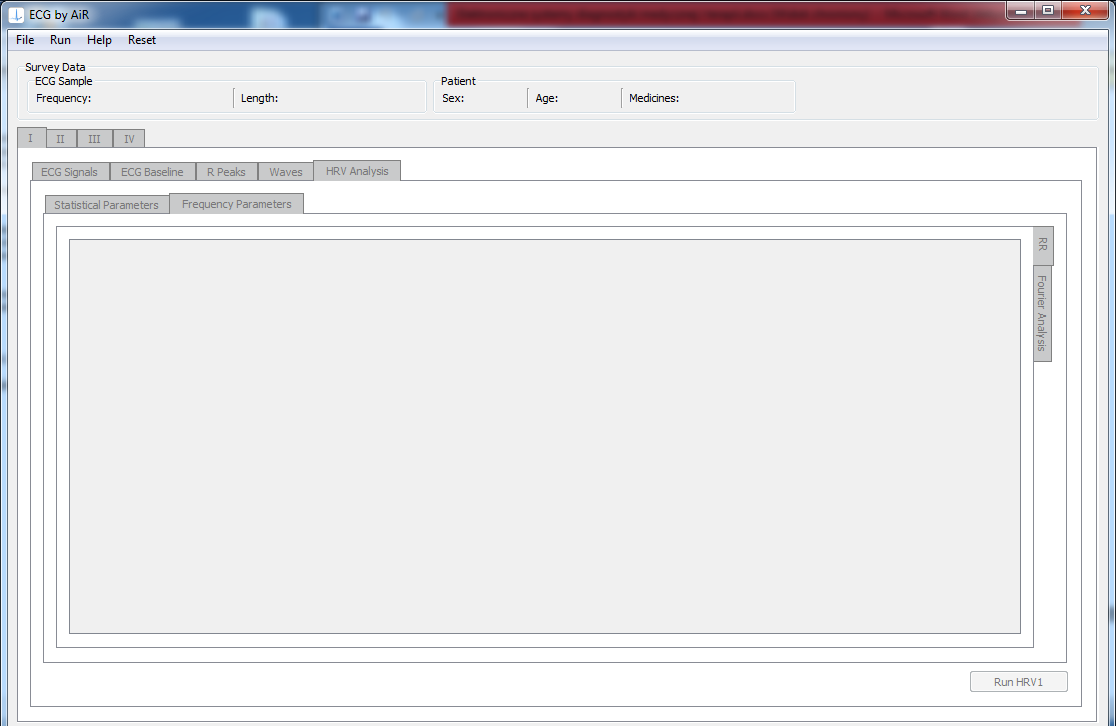
\includegraphics[width=\textwidth]{GUI/img/okno_g}
\label{fig:okno_gi}
\caption{Okno główne programu.}
\end{figure}

Na górze okna głównego znajduje się Menu aplikacji, o następującej strukturze:

\begin{itemize}
\item File
\begin{itemize}
\item Open
\item Exit
\end{itemize}
\item Run
\begin{itemize}
\item Run ECG Baseline
\item Run R Peaks
\item Run Waves
\item HRV Analysis
\item QRS Classification
\item HRT Analysis
\item ST Segment
\item VCG Loop
\item Sig EDR
\item Atrial Fibr
\item QT Disp
\item Sleep apnea
\item RUN ALL
\end{itemize}
\item Help
\begin{itemize}
\item About
\end{itemize}

Opcja File -> Open powoduje uruchomienie okna dialogowego filebrowser, w którym możliwe jest wybranie zestawu danych do przetwarzania.

\begin{figure}[H]
\centering
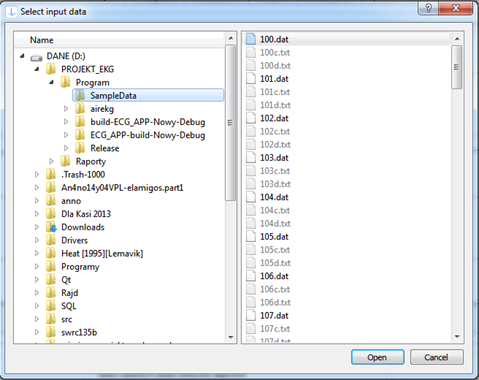
\includegraphics[width=\textwidth]{GUI/img/file_b}
\label{fig:file_b}
\caption{Wybór pliku z danymi.}
\end{figure}

Opcje z grupy Run służą do wywoływania poszczególnych modułów przetwarzających sygnał EKG. Ostatnią z opcji jest RUN ALL wybranie jej powoduje uruchomienie wszystkich modułów EKG w odpowiedniej kolejności. Podczas obliczania odpowiedzi, w dolnej części ekranu pokazywany jest pasek informujący o trwającym przetwarzaniu sygnału.

W grupie Help znajduje się opcja About powoduje ona uruchomienie okna dialogowego, zawierającego informacje o twórcach programu.

Poniżej menu znajdują się pola zawierające dane o sygnale EKG oraz badanym pacjencie: 

\begin{itemize}
\item Częstotliwość pomiaru (Frequency)
\item Długość pomiaru (Length)
\item Płeć (Sex) 
\item Wiek (Age)
\item Przyjmowane leki (Medicines)
\end{itemize}

Po wczytaniu danych, centralną część ekranu zajmuje wykres, przedstawiający sygnał EKG, za pomocą zakładek znajdujących się nad nim  możemy przechodzić do poszczególnych modułów. Moduły zostały podzielone na 4 zakładki w celu ułatwienia poruszania się po programie. W zależności od wybranego modułu, pod wykresem, znajdują się dostępne opcje konfiguracyjne. W każdej zakładce znajduje się przycisk Run pozwalający odpalić konkretny moduł, zaś na dole ekrany do dyspozycji użytkownika jest przycisk RUN ALL uruchamiający wszystkie moduły.